\newcommand\gax{
  \begin{center}
    \begin{tikzpicture}[scale=0.85]
      % horizontal extent ensures left edge at x=-5 aligns with structure below
      \draw[->] (-5,0) -- (5,0) node[above right] {$x$};
      \draw[->] (-5,-1.1) -- (-5,1.1) node[left] {$g_z$};
      \draw[dashed,gray] (-5,0) -- (5,0);
      %\node[align=left] at (2.8,1.0) {\small Sketch $g_z(x)$ \\[-2pt] \small (assume $\Delta\rho>0$)};
    \end{tikzpicture}
  \end{center}
}

\begin{activity}{Geologic Structures to Gravity Anomalies}

\section*{Purpose}

To develop intuition for how geological structures are represented by idealized geometric bodies in gravity interpretation. By relating common geologic features to simple analytical models, you will explore how density contrast, geometry, and burial depth influence the character of gravity anomalies.

\section*{Learning Outcomes}

By the end of this activity, you should be able to:

\begin{itemize}
  \item identify geological structures that can be approximated by common gravity-model geometries,
  \item estimate plausible density contrasts for a variety of lithologies and geologic settings,
  \item predict the qualitative shape of gravity anomalies from simple subsurface structures,
  \item relate anomaly symmetry, width, amplitude, and gradients to source geometry,
  \item explain the advantages and limitations of using simplified geometric models in gravity interpretation.
\end{itemize}

\section*{Introduction}

The structural arrangement of rock units can be very complex.  As geophysicists we invert for more complex structures as necessary, but doing so is time-consuming.  We can often approximate complex structures by one or more simplified geometries.  These simplifications have benefits besides being faster.  For one, the models have closed form analytical solutions.  We can calculate a wide range of stuctures that vary in dimension, distance, or orientation rapidly giving us approximate solutions that in many cases are `good enough' given all the data uncertainties and model non-uniqueness issues.  Another advantage is that closed form solutions help build our intution in a way that inverting for cell properties do not.

\section*{Task}
For each structure below, complete the table and use the \emph{upper axes} to sketch the expected gravity anomaly $g_z(x)$ (arbitrary units).  The \emph{lower panel} shows a schematic cross-section ($z$ positive downward).  Assume that structures extend into and out of the page (i.e., perpendicular to strike).\\

In your groups:
\begin{enumerate}
  \item Discuss geologic structures that may be described by the simple shapes.
  \item Propose plausible density contrasts ($\Delta\rho$) given typical lithologies.
  \item Predict qualitative anomaly shape: narrow/broad? symmetric/asymmetric? positive/negative? asymptotic limit?
  \item One group presents each structure; whole class discusses similarities and differences.
\end{enumerate}

{\small
\begin{tblr}{
  colspec = {cX[c]X[c]c},
  row{4-10} = {ht=2.5em},
  hline{1,4,11} = {solid},
  hline{5-10} = {dashed},
  vline{1,5} = {solid},
  vline{2-4} = {dashed}
}
  & & & \textbf{Plausible Range} \\
  & \textbf{Geologic Structure(s)} & \textbf{Likely lithologies} & $\Delta\rho$ \\
  & & & (kg m$^{-3}$) \\
  A. & & & \\
  B. & & & \\
  C. & & & \\
  D. & & & \\
  E. & & & \\
  F. & & & \\
  G. & & & \\
\end{tblr}
}

\vspace{0.75em}
\noindent\textbf{Prompts:} Indicate sign (pos./neg.), width (narrow/broad), symmetry/asymmetry, and where the steepest gradients occur.

\bigskip\bigskip

% ==========================================================
% A) Buried Sphere (3D)
% ==========================================================
\begin{center}
\textbf{A) Cylinder}
\end{center}

% --- Anomaly axes (aligned with left edge) ---
\gax

% --- Cross-section (no vertical axis) ---
\begin{center}
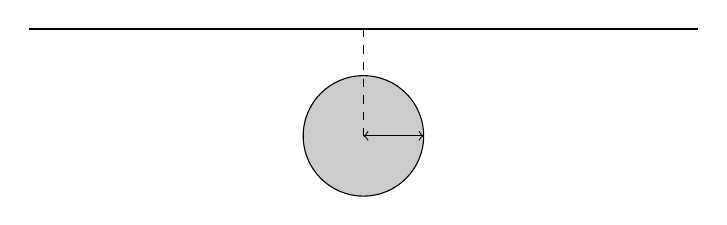
\begin{tikzpicture}[scale=0.85]
  \draw[thick] (-5,0) -- (5,0); % surface only
  % Sphere
  \def\xc{0} \def\zc{-1.6} \def\r{0.9}
  \draw[fill=gray!40] (\xc,\zc) circle (\r);
  \draw[dashed] (\xc,0) -- (\xc,\zc);% node[midway,right] {$z_0$};
  \draw[<->] (\xc+\r,\zc) -- (\xc,\zc);% node[midway,below] {$a$};
\end{tikzpicture}
\end{center}

\bigskip\bigskip

% ==========================================================
% B) Laccolith
% ==========================================================
\begin{center}
\textbf{B) Sigmoid}
\end{center}

\gax

\begin{center}
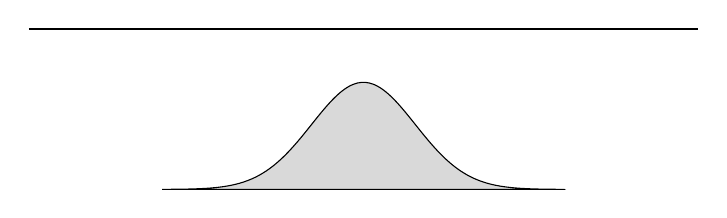
\begin{tikzpicture}[scale=0.85]
  \draw[thick] (-5,0) -- (5,0); % surface

  \draw[fill=gray!30]
    plot[
      domain=-3:3,
      samples=100,
      smooth
    ]
    (\x,{-(2.4-1.6*exp(-0.5*\x*\x/0.6))})
    -- (3,-2.4)
    -- (-3,-2.4)
    -- cycle;
\end{tikzpicture}
\end{center}

% \begin{center}
% \begin{tikzpicture}[scale=0.85]

%   % surface
%   \draw[thick] (-5,0) -- (5,0);

%   % parameters
%   \def\xc{0}
%   \def\zc{-1.3}
%   \def\r{0.7}
%   \def\rb{0.6}
%   \def\depth{0.35} % visual "3-D" depth
%   \def\p{0.8}


%   % side walls
%   %\draw[fill=gray!50]
%   %  (\xc-\r,\zc) -- (\xc-\r-\depth,\zc-\depth)
%   %  arc (180:0:{\r} and {0.35})
%   %  -- (\xc+\r,\zc)
%   %  arc (0:180:{\r} and 0.35);

%   % back ellipse
%   \draw[fill=gray!30] (\xc+\depth*2,\zc+\depth/2) ellipse ({\rb*\p} and {\r*\p});

%   % side walls
%   \fill[gray!30] (\xc-\depth*2,\zc-\depth/2-\r) -- (\xc-\depth*2,\zc-\depth/2+\r) -- (\xc+\depth*2,\zc+\depth/2+\r*\p) -- (\xc+\depth*2,\zc+\depth/2-\r*\p) -- cycle;
%   \draw (\xc+\depth*2,\zc+\depth/2-\r*\p) -- (\xc-\depth*2,\zc-\depth/2-\r) -- (\xc-\depth*2,\zc-\depth/2+\r) -- (\xc+\depth*2,\zc+\depth/2+\r*\p);


%   % front ellipse
%   \draw[fill=gray!30] (\xc-\depth*2,\zc-\depth/2) ellipse ({\rb} and {\r});

%   % depth to center
%   \draw[dashed] (\xc,0) -- (\xc,\zc);% node[midway,right] {$z_0$};
%   \draw[dashed] (\xc+\depth*2,\zc+\depth/2) -- (\xc-\depth*2,\zc-\depth/2);

%   % label
%   %\node at (3.0,-2.6) {\small infinite strike out of page};

%\end{tikzpicture}
%\end{center}

\bigskip\bigskip

% ==========================================================
% C) Vertical Dike
% ==========================================================
\newpage
\begin{center}
\textbf{C) Vertical Slab}
\end{center}

\gax

\begin{center}
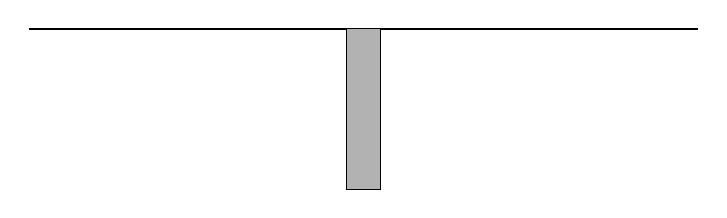
\begin{tikzpicture}[scale=0.85]
  \draw[thick] (-5,0) -- (5,0);
  \draw[fill=gray!60] (-0.25,0) rectangle (0.25,-2.4);
  %\draw[dashed] (0,0) -- (0,-2.4) node[midway,right] {depth};
  %\draw[<->] (-0.25,-2.6) -- (0.25,-2.6) node[midway,below] {width};
\end{tikzpicture}
\end{center}

\bigskip\bigskip

% ==========================================================
% D) Finite-Extent Sill
% ==========================================================
\begin{center}
\textbf{D) Finite-Extent Horizontal Slab}
\end{center}

\gax

\begin{center}
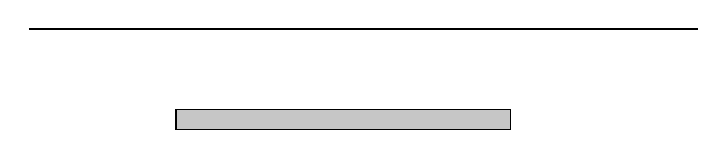
\begin{tikzpicture}[scale=0.85]
  \draw[thick] (-5,0) -- (5,0);
  \draw[fill=gray!45] (-2.8,-1.2) rectangle (2.2,-1.5);
  %\draw[dashed] (0,0) -- (0,-1.2) node[midway,right] {depth to top};
  %\draw[<->] (-2.8,-1.7) -- (2.2,-1.7) node[midway,below] {extent};
  %\draw[<->] (2.5,-1.2) -- (2.5,-1.5) node[midway,right] {thickness};
\end{tikzpicture}
\end{center}

\bigskip\bigskip

% ==========================================================
% E) Inclined Dike
% ==========================================================
\begin{center}
\textbf{E) Inclined Plane}
\end{center}

\gax

\begin{center}
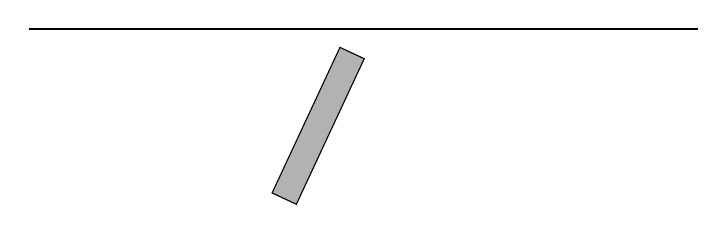
\begin{tikzpicture}[scale=0.85]
  \draw[thick] (-5,0) -- (5,0);
  % Inclined dike, dip ~25°
  \begin{scope}[rotate=-25]
    \draw[fill=gray!60] (-0.2,-0.4) rectangle (0.2,-2.8);
  \end{scope}
  %\node at (2.8,-2.5) {\small dip $\sim 25^\circ$};
\end{tikzpicture}
\end{center}

\bigskip\bigskip

% ==========================================================
% F) Faulted Contact (60° dip) with equal thickness layer displaced
% ==========================================================
\begin{center}
\textbf{F) Offset Layer}
\end{center}

% --- Anomaly axes (aligned) ---
\gax

% --- Cross-section with 60° dipping fault and displaced layer of constant thickness ---
\begin{center}
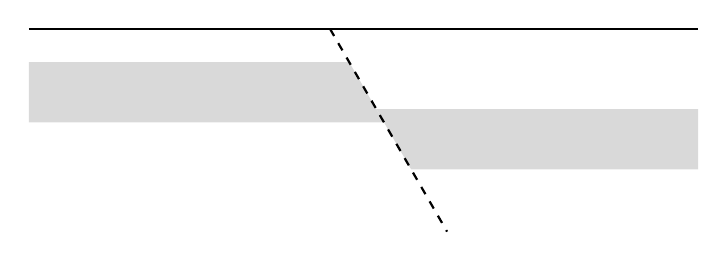
\begin{tikzpicture}[scale=0.85]
  % --- Surface ---
  \draw[thick] (-5,0) -- (5,0);

  % --- Parameters ---
  \def\xf{-0.5}    % surface fault x-position
  \def\dip{60}     % fault dip (degrees), dipping to the right
  \def\tlay{0.9}   % layer thickness (constant on both sides)
  \def\ztopL{-0.5} % top of layer on left (upthrown) side (negative = below surface)
  \def\ztopR{-1.2} % top of layer on right (downthrown) side

  % --- Trig helpers ---
  \pgfmathsetmacro{\cosd}{cos(\dip)}
  \pgfmathsetmacro{\sind}{sin(\dip)}
  \pgfmathsetmacro{\cotd}{\cosd/\sind}

  % =========================
  % Left block intersections
  % =========================
  % Left top and base depths
  \pgfmathsetmacro{\zLt}{\ztopL}               % z top (left)
  \pgfmathsetmacro{\zLb}{\ztopL - \tlay}       % z base (left)
  % Intersections with dipping fault: x = xf - z * cot(dip)
  \pgfmathsetmacro{\xLt}{\xf - (\zLt)*\cotd}   % x at top-left vs fault
  \pgfmathsetmacro{\xLb}{\xf - (\zLb)*\cotd}   % x at base-left vs fault

  % =========================
  % Right block intersections
  % =========================
  \pgfmathsetmacro{\zRt}{\ztopR}               % z top (right)
  \pgfmathsetmacro{\zRb}{\ztopR - \tlay}       % z base (right)
  \pgfmathsetmacro{\xRt}{\xf - (\zRt)*\cotd}   % x at top-right vs fault
  \pgfmathsetmacro{\xRb}{\xf - (\zRb)*\cotd}   % x at base-right vs fault

  % --- Left block (upthrown): layer polygon extends to the dipping fault ---
  % Vertices (counter-clockwise): left boundary top -> fault at top -> fault at base -> left boundary base
  \path[fill=gray!30,draw=none]
       (-5,\zLt) -- (\xLt,\zLt) -- (\xLb,\zLb) -- (-5,\zLb) -- cycle;

  % --- Right block (downthrown): same thickness, shifted down; also extends to the fault ---
  % Vertices: fault at top -> right boundary top -> right boundary base -> fault at base
  \path[fill=gray!30,draw=none]
       (\xRt,\zRt) -- (5,\zRt) -- (5,\zRb) -- (\xRb,\zRb) -- cycle;

  % --- Fault trace from surface: show a clear dipping plane ---
  % long dashed line down-dip; a short up-dip stub (optional)
  \draw[dashed,thick] (\xf,0) -- ++({ 3.5*\cosd},{-3.5*\sind});
  %\draw[dashed]       (\xf,0) -- ++({-1.2*\cosd},{ 1.2*\sind});

  % --- Labels ---
  %\node at (-3.7,-0.25) {\small upthrown side};
  %\node at (3.2,-0.95)  {\small downthrown side};
  %\node[rotate=-\dip] at (\xf+1.0,-0.8) {\small fault $60^\circ$};

  % Optional thickness arrows on each side
  %\draw[<->] (-4.6,\zLt) -- (-4.6,\zLb) node[midway,left]  {\small thickness};
  %\draw[<->] ( 4.6,\zRt) -- ( 4.6,\zRb) node[midway,right] {\small thickness};
\end{tikzpicture}
\end{center}

\bigskip\bigskip

% ==========================================================
% G) Gently Sloped Basin with edge at one-third from left boundary
% ==========================================================
\newpage
\begin{center}
\textbf{G) Gently Sloped Basin (edge at one-third from left boundary)}
\end{center}

% --- Anomaly axes (aligned) ---
\gax

% --- Cross-section: edge located at one-third from left (i.e., x = -5 + (10/3) ≈ -1.667) ---
\begin{center}
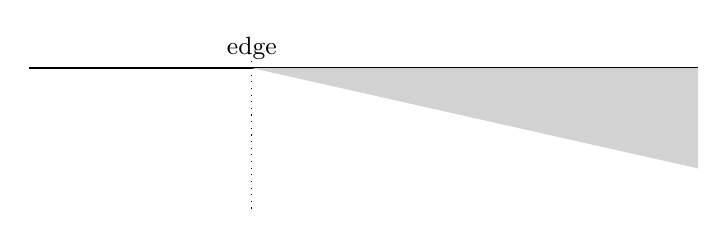
\begin{tikzpicture}[scale=0.85]
  \draw[thick] (-5,0) -- (5,0);
  % Geometry
  \def\xL{-5}
  \def\xR{5}
  \def\xEdge{-1.6667} % one-third from left
  %\def\zThin{-0.6}
  %\def\zThick{-2.0}
  \def\zThin{0.0}
  \def\zThick{-1.5}
  % Polygon: start thin on left, thicken rightward after the edge
  % Left triangle/wedge up to the edge
  %\fill[gray!35] (\xL,\zThin) -- (\xL,0) -- (\xEdge,0) -- (\xEdge,\zThin) -- cycle;
  % Right wedge thickening from the edge to the right boundary
  \fill[gray!35] (\xEdge,\zThin) -- (\xEdge,0) -- (\xR,0) -- (\xR,\zThick) -- cycle;
  % Labels
  %\node at (3.0,-0.3) {\small thicker sediments to the right};
  \draw[dotted] (\xEdge,0.1) -- (\xEdge,-2.1);
  \node at (\xEdge,0.3) {\small edge};
\end{tikzpicture}
\end{center}

\bigskip\bigskip

\section*{Key Ideas}

\textbf{Anomaly width reflects source depth.} Shallower bodies produce narrower, sharper anomalies; deeper bodies produce broader, smoother anomalies. This depth--wavelength relationship is a fundamental constraint on gravity interpretation.

\begin{figure}[h]
\centering
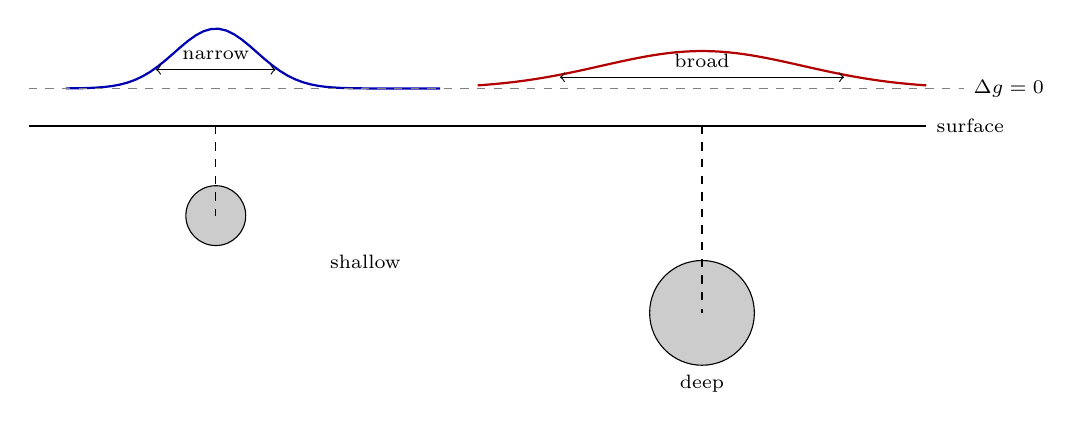
\begin{tikzpicture}[scale=0.95]
  % Surface line
  \draw[thick] (-6, 3.5) -- (6, 3.5) node[right, font=\scriptsize] {surface};

  % Shallow sphere
  \draw[fill=gray!40] (-3.5, 2.3) circle (0.4);
  \draw[dashed] (-3.5,3.5) -- (-3.5,2.3);
  \node[font=\scriptsize, below] at (-1.5,1.9) {shallow};

  % Deep sphere
  \draw[fill=gray!40] (3.0, 1.0) circle (0.7);
  \draw[dashed] (3.0,3.5) -- (3.0,1.0);
  \node[font=\scriptsize, below] at (3.0,0.3) {deep};

  % Anomaly curves (schematic above surface)
  \begin{scope}[yshift=4.0cm]
    % Narrow, peaked (shallow)
    \draw[blue!70!black, thick] plot[domain=-5.5:-0.5, samples=50]
      (\x, {0.8*exp(-0.5*(\x+3.5)^2/0.3)});
    \draw[<->] (-4.3, 0.25) -- (-2.7, 0.25)
      node[midway, above, font=\scriptsize] {narrow};

    % Broad, smooth (deep)
    \draw[red!70!black, thick] plot[domain=-0:6, samples=60]
      (\x, {0.5*exp(-0.5*(\x-3.0)^2/1.8)});
    \draw[<->] (1.1, 0.15) -- (4.9, 0.15)
      node[midway, above, font=\scriptsize] {broad};

    \draw[dashed, gray] (-6,0) -- (6.5,0);
    \node[right, font=\scriptsize] at (6.5, 0) {$\Delta g=0$};
  \end{scope}
\end{tikzpicture}
\caption{Shallower bodies produce narrower, higher-amplitude anomalies; deeper bodies produce broader, lower-amplitude anomalies with the same total mass excess. Anomaly half-width $\approx$ depth to source.}
\end{figure}

\textbf{Anomaly sign reflects density contrast.} Bodies denser than their surroundings ($\Delta\rho > 0$) produce positive anomalies; bodies less dense than their surroundings produce negative anomalies.

\textbf{Symmetry reveals geometry.} Symmetric anomalies suggest symmetric bodies (sphere, vertical dike); asymmetric anomalies indicate asymmetric structures (inclined plane, faulted contact). The location and sign of the steepest gradient constrain the lateral position and dip of the source edge.

\textbf{Non-uniqueness is unavoidable.} Different geometries with appropriate density contrasts can produce identical surface gravity anomalies. Additional constraints (geology, seismic data, drill-hole information) are always needed to discriminate between alternative models.


\end{activity}